\chapter{Модель гистерезисного микроансамбля} \label{chapter:neuron}

В главе даётся формальное определение модели нейрона в виде системы обыкновенных дифференциальных уравнений, а так же определяется понятие микроансамбля --- сильно связного объединения нейронов. Анализируются точки равновесия и проводится бифуркационный анализ модели микроансамбля с применением двух различных функций активации: \textit{оригинальной} и \textit{сигмоидальной}. Полученные частные результаты обобщаются на случай целого класса функций активации, которые обеспечивают наличие характерной поведенческой динамики. В результате, определяются основные понятия и свойства, связанные с предлагаемой моделью, а так же моделируются типичные сценарии функционирования простой модели микроансамбля.

%==============================================================================
%                          Формальное определение модели
%==============================================================================
\section{Формальное определение} \label{section:neuron_model}

Основой для рассматриваемой в диссертационной работе модели нейрона послужила монография~\cite{EmelyanovYaroslavsky1990}, в которой описан подход к построению искусственной \acr{NN}, потенциально обладающей интеллектуальными свойствами и названной автором \textit{индуктивным автоматом}. Особенность работы заключается в том, что автор предлагает оригинальную модель нейрона и показывает через численные и умозрительные эксперименты, что благодаря ряду локальных свойств совокупность нейронов способна демонстрировать нетривиальное поведение. Однако предложенная модель индуктивного автомата носит ярко выраженный незаконченный характер и кроме того, преследует целью биологическую правдоподобность, что так же отразилось на сложности модели.

Данная диссертационная работа направлена на получение потенциальной прикладной значимости, в частности, при решении задачи контекстно-зависимого распознавания образов. Поэтому предложенный в работе~\cite{EmelyanovYaroslavsky1990} подход был в значительной мере переосмыслен и в результате была выработана собственная нейросетевая модель: она не содержит биологически обоснованных и стохастических элементов, а так же в противоположность \textit{Integrate-And-Fire} типу модели, где подразумевается моделирование на уровне отдельных импульсов нейрона с частотно-фазовым кодированием информации, является более классической \textit{Firing-Rate}  моделью~\cite{Dayan2001}, в которой выходным параметром нейрона является \socalled частота --- усреднённая по времени частота генерации импульсов. И хотя первый тип обладает более разнообразной поведенческой динамикой и информационной ёмкостью~\cite{Izhikevich2006}, практическое применение этого типа моделей сопряжено с рядом проблем, включая сложность их анализа и вычислительную дороговизну.

Таким образом, формальная модель нейрона приобрела следующий вид:
\begin{equation}
	\label{eq:full_single_neuron_model}
    \begin{cases}
        d\scalar{u} / d\scalar{t}   &=  \vector{w}^{\top} \vector{x} - \scalar{p} - \mu \scalar{u}, \\
        \scalar{y}                  &=  f\left( h\left( \scalar{u}, \theta \right) \right), \\
    \end{cases}
\end{equation}
где $\scalar{u} \in \specialset{R}$ --- потенциал нейрона (внутреннее состояние), $\vector{x} \in \specialset{R}^{M}$ -- входной вектор нейрона (входной сигнал), $\vector{w} \in \specialset{R}^{M}$ --- вектор весовых коэффициентов нейрона,  $\scalar{p}$ --- внутренний порог нейрона, $\mu \in \left(0;1\right)$ --- константа диссипации, характеризующая скорость убывания потенциала нейрона, $\scalar{y} \in \left[0;1\right]$ --- частота нейрона (выходной сигнал), $\theta \in \specialset{R}^{+}$ --- управляющий параметр сети, который будет рассмотрен более подробно в следующих главах.

Функция \textit{модуляции} $h: \specialset{R} \times \specialset{R}^{+} \to \specialset{R}$ преобразует потенциал нейрона $\scalar{u}$ в соответствии со значением управляющего параметра $\theta$ следующим образом:
\begin{equation}
    \label{eq:h_function}
    h\left( \scalar{u}, \theta \right) = \scalar{u} / \theta.
\end{equation}

Функция \textit{активации} $f: \specialset{R} \to \left[0;1\right]$ преобразует модулированный потенциал нейрона $h\left( \scalar{u}, \theta \right)$ в выходную частоту $\scalar{y}$. В данной главе будут рассмотрены две функции активации, которые изображены \onfigure~\ref{fig:model_activation_functions}:
\begin{itemize}
	\item \textit{Оригинальная} функция активации $f_{s}$, полученная на основе функции динамического порога $\text{П}^\text{Д}$ из работы~\cite{EmelyanovYaroslavsky1990}. Отметим, что использовать непосредственно функцию $\text{П}^\text{Д}$ невозможно, т.к. её аргументом является межимпульсный интервал и, что важнее, автором не была задана её аналитическая форма. Подробно процесс приведения данной функции к приемлемому для нас виду изложен \inappendix~\ref{appendix:activation_function} \inquotes{\nameref{appendix:activation_function}} --- в результате, было получено следующее выражение:
		\begin{equation}
            \label{eq:activation_function_original}
            f_{s}(\scalar{u}) = 
            \begin{cases}
                0                                                                               &, \scalar{u} < u_{01} \\
                0,1935 + \dfrac{1}{120} \ln\left( \dfrac{\scalar{u}}{2,6 - \scalar{u}} \right)  &, u_{01} \le \scalar{u} \le u_{12} \\
                1 - \dfrac{z_{12}}{\scalar{u} - k_{12}}                                         &, \scalar{u} > u_{12} \\
            \end{cases}
		\end{equation}
        а значения коэффициентов определяются как:
        \begin{align*}
            &z_{12} = 177,84 \cdot \sigma\left(6,18\right) \cdot \left(1 - \sigma\left(6,18\right)\right) \approx 0,37, \\
            &k_{12} = 2,6 \cdot \sigma\left(6,18\right) - z_{12} / 0,755 \approx 2,11, \\
            &u_{01} = 2,6 \cdot \sigma\left(-23,22\right) \approx 0, \\
            &u_{12} = 2,6 \cdot \sigma\left(6,18\right) \approx 2,6,
        \end{align*}
        где $\sigma$ --- логистическая функция.
	\item \textit{Сигмоидальная} функция активации $f_{\sigma}$, которая получила широкое распространение в области нейронных сетей, нечёткой логики и \other, заданная следующим образом:
		\begin{equation}
            \label{eq:activation_function_sigma}
			f_{\sigma}(\scalar{u}) = \dfrac{1}{1 + e^{\displaystyle -(\scalar{u} - 3)}}.
		\end{equation}
\end{itemize}

\IncludeFigure[t]{model_activation_functions}{Вид оригинальной $f_{s}$ и сигмоидальной $f_{\sigma}$ функций активации.}

Для удобства дальнейшего изложения мы применим приём, который часто используется в области нейросетевого моделирования: положим, что $\vectoritem{x}{0}$ в любой момент времени равно $1$, а $\vectoritem{w}{0}$ равен $-\scalar{p}$, тогда выражение~\eqref{eq:full_single_neuron_model} можно записать в более компактной эквивалентной форме:
\begin{equation}
    \label{eq:single_neuron_model}
    \begin{cases}
        d\scalar{u} / d\scalar{t}   &=  \vector{w}^{\top} \vector{x} - \mu \scalar{u}, \\
        \scalar{y}                  &=  f\left( h\left( \scalar{u}, \theta \right) \right), \\
    \end{cases}
\end{equation}
которая будет использована далее наравне с выражением~\eqref{eq:full_single_neuron_model}.

\begin{Definition}
    Будем называть \textit{микроансамблем} математическую структуру $A = \left\{ \customset{N}, \matrix{V} \right\}$, где $\customset{N} = \left\{ n_{i} \right\}_{i=1}^{N} $ --- множество нейронов, составляющих микроансамбль, и $\matrix{V}_{N \times N}$ --- матрица, задающая топологию и коэффициенты связей между нейронами микроансамбля. При этом размер множества $\customset{N}$ и элементы матрицы $\matrix{V}$ фиксированы, \ie не меняются в процессе обучения и функционирования сети, и выбираются заранее, исходя из требуемых вычислительных свойств микроансамбля как целостной вычислительной единицы \acr{NN}.
\end{Definition}

Основываясь на выражении~\eqref{eq:single_neuron_model}, динамика микроансамбля может быть описана следующим образом:
\begin{equation}
    \label{eq:microensemble_model}
    \begin{cases}
        d\vector{u}/d\scalar{t} &= \matrix{V}^{\top} \vector{y} + \matrix{W}^{\top} \vector{x} - \mu \vector{u}, \\
        \vector{y}              &= f\left( h\left( \vector{u}, \theta \right) \right), \\
    \end{cases}
\end{equation}
где все параметры и переменные имеют тот же смысл, что и в выражении~\eqref{eq:single_neuron_model}, но записанные в векторно-матричной форме, а матрица $\matrix{W}_{M \times N} = \left[ \vector{w}_{1} \ldots \vector{w}_{N} \right]$, составленная из векторов-столбцов $\vector{w}_{i}$, отражает связи входного вектора $\vector{x}$ со всеми нейронами микроансамбля.

Для дальнейшего анализа и выявления характерных свойств модели микроансамбля, которые затем позволят оценить её с точки зрения вычислительного элемента \acr{NN}, введём понятие простого микроансамбля.
\begin{Definition}
    Будем называть микроансамбль $A$ \textit{простым микроансамблем}, если выполнены следующие условия:
    \begin{itemize}
        \item все нейроны микроансамбля соединены друг с другом связями весом $\omega$, \ie: $\matrix{V}_{N\!\times\!N} = \omega \cdot \left( \matrix{J}_{N\!\times\!N} - \matrix{I}_{N} \right)$, где матрицы $\matrix{J}$ и $\matrix{I}$  --- матрица единиц и единичная матрица соответственно;
        \item все нейроны микроансамбля имеют одинаковые связи с входным вектором $\vector{x}$, \ie: $\forall\ i \in \overline{1,N}\ \vector{w}_{i} = \vector{w}$;
        \item начальные условия для всех нейронов микроансамбля совпадают, \ie: \par $\vector{u}_{t=0} = \scalar{u}^{0} \cdot \matrix{J}_{N\!\times\!1}$, где $\scalar{u}^{0}$ --- начальное значение потенциала.
    \end{itemize}
\end{Definition}

В этом случае можно говорить об эквивалентности всех нейронов микроансамбля, а значит всё множество нейронов $\customset{N}$ может быть представленно одним гипер-нейроном с рекуррентной связью на себя, как показано \onfigure~\ref{fig:model_simple_microensemble}. Выражение~\eqref{eq:microensemble_model} при этом примет следующий вид:
\begin{equation}
    \label{eq:simple_microensemble_model}
    \begin{cases}
        d\scalar{u}/d\scalar{t} &= \alpha \scalar{y} + \vector{w}^{\top} \vector{x} - \mu \scalar{u}, \\
        \scalar{y}              &= f\left( h\left( \scalar{u}, \theta \right) \right), \\
    \end{cases}
\end{equation}
где параметр $\alpha = \omega \cdot \left( N - 1 \right)$ --- весовой коэффициент рекуррентной связи, который по смыслу отражает связность нейронов микроансамбля. Выражение~\eqref{eq:simple_microensemble_model} так же можно представить в более простой форме, близкой к той, что используется при описании рекуррентных моделей нейронов в нейродинамике~\cite{Haykin2008}:
\begin{equation}
    \label{eq:simple_microensemble_model_plain}
    d\scalar{u}/d\scalar{t} = \alpha f\left( h\left( \scalar{u}, \theta \right) \right) + \vector{w}^{\top} \vector{x} - \mu \scalar{u}.
\end{equation}
Однако запись в виде системы более удобна в том смысле, что явно содержит выходную переменную $y$.

\IncludeFigure[t]{model_simple_microensemble}{Приведение простого микроансамбля с 3-мя нейронами к виду эквивалентного гипер-нейрона с рекуррентной связью $\alpha$ на себя.}

Стоит отметить, что в работе~\cite{Pchelkin2003} исследовалась похожая на систему~\eqref{eq:simple_microensemble_model} модель нейронного ансамбля, которая так же была основана на развитии модели индуктивного автомата~\cite{EmelyanovYaroslavsky1990}. Однако автор, во-первых, не учитывал внешнее влияние на нейроны (слагаемое $\vector{w}^{\top} \vector{x}$), и во-вторых, был сосредоточен на конкретной проблеме, а именно на связи поведения модели с \socalled оптимальной частотой --- основополагающим параметром модели индуктивного автомата, который в явном виде отсутствует в рассматриваемой нами модели.


%==============================================================================
%                   Точки равновесия и бифуркационный анализ
%==============================================================================
\section{Точки равновесия и бифуркационный анализ} \label{section:neuron_equilibrium}

Для удобства дальнейшего анализа введём величину $\scalar{i} = \vector{w}^{\top} \vector{x}$ --- внешнее возбуждение микроансамбля, и обозначим правую часть дифференциального уравнения системы~\eqref{eq:simple_microensemble_model} как:
\begin{equation}
    \label{eq:functional_u}
    F(\scalar{u}) = \alpha f\left( h\left( \scalar{u}, \theta \right) \right) + \scalar{i} - \mu \scalar{u}.
\end{equation}
Сразу отметим, что в такой форме записи выходная переменная $y$ присутствует неявно через переменную $u$. Однако, применяя определение переменной $\scalar{y}$ из системы~\eqref{eq:simple_microensemble_model} и определение функции $h$~\eqref{eq:h_function}, данную функцию можно переписать в виде:
\begin{equation}
    \label{eq:functional_y}
    F(\scalar{y}) = \alpha \scalar{y} + \scalar{i} - \mu \theta g(\scalar{y}),
\end{equation}
где переменная $y$ присутствует уже явно, а $g$ --- обратная функция к $f$. Для рассматриваемых нами функций активации обратные будут определяться следующим образом:
\begin{itemize}
    \item Для \textit{оригинальной} функции $f_{s}$, заданной выражением~\eqref{eq:activation_function_original}:
    \begin{equation}
        \label{eq:unactivation_function_original}
        g_{s}(\scalar{y}) = 
        \begin{cases}
            \dfrac{2,6}{1 + e^{\displaystyle -120 \cdot (\scalar{y} - 0,1935)}} &, y \in \left(0; y_{12}\right] \\
            k_{12} + \dfrac{z_{12}}{1 - \scalar{y}}                             &, y \in \left(y_{12}; 1\right] \\
        \end{cases}
    \end{equation}
    где $y_{12} = 0,245$, а точке $y = 0$ соответствует интервал $\left(-\infty; u_{01}\right]$.
    \item Для \textit{сигмоидальной} функции $f_{\sigma}$, заданной выражением~\eqref{eq:activation_function_sigma}:
    \begin{equation}
        \label{eq:unactivation_function_sigma}
        g_{\sigma}(\scalar{y}) = 3 + \ln\left(\dfrac{\scalar{y}}{1 - \scalar{y}}\right),\;y \in \left[0; 1\right].
    \end{equation}
\end{itemize}

Для нахождения устойчивых точек системы~\eqref{eq:simple_microensemble_model}, описывающей динамику простого микроансамбля, необходимо найти корни уравнения $F = 0$. Однако для рассматриваемых нами функций активации сделать это аналитически невозможно, т.к. при этом в выражениях~\eqref{eq:functional_u} и~\eqref{eq:functional_y}, определяющих функцию $F$, переменная будет одновременно встречаться в основании и показателе степени. Поэтому будем рассматривать решение графически, причём в виде пересечения двух кривых, приравняв выражение~\eqref{eq:functional_y} к нулю и переписав результат следующим образом:
\begin{equation}
    \label{eq:graphic_solution}
    \scalar{i} = - \alpha \scalar{y} + \mu \theta g(\scalar{y}),
\end{equation}
где прямая в левой части равенства отражает внешнее воздействие на микроансамбль, а кривая в правой --- внутреннюю динамику микроансамбля. Такая форма решения более удобна по сравнению с непосредственным изображением функции $F$, т.к. позволяет наглядно продемонстрировать соответствие между выходной частотой $\scalar{y}$ и внешним возбуждением $\scalar{i}$, которое в свою очередь является линейной комбинацией компонент входного вектора $\vector{x}$.

При этом ещё раз отметим, что параметры $i$ и $\theta$ меняются в процессе функционирования сети, в то время как параметр $\alpha$ подбирается и фиксируется заранее, так же как и константа диссипации $\mu$.

%==============================================================================
\subsection{Модель с сигмоидальной функцией активации} \label{subsection:analysis_sigm}

Сперва рассмотрим более простой вариант модели с \textit{сигмоидальной} функцией активации (\acr{SAF}-модель). На рисунке~\ref{fig:analysis_sigm_equilibriums} приведены графические решения системы~\eqref{eq:simple_microensemble_model} согласно выражению~\eqref{eq:graphic_solution} и соответствующие графики функции $F(\scalar{y})$ для двух типичных наборов значений параметров: а) $\mu = 0,75$, $\alpha = 1,0$, $\theta = 1$, $p = 1,25$ и $i = 3$; б) $\mu = 0,75$, $\alpha = 5,0$, $\theta = 1$, $p = 1,25$ и $i = 1$.
\IncludeFigure[t]{analysis_sigm_equilibriums}{Графическое решение системы~\eqref{eq:simple_microensemble_model} и график функции $F(\scalar{y})$ для случаев: а) с одной точкой устойчивого равновесия $\scalar{y}^{*}$; б) с одной точкой неустойчивого равновесия $\scalar{y}_{2}^{*}$ и двумя точками $\scalar{y}_{1,3}^{*}$ -- устойчивого.}
Как будет показано в дальнейшем аналитически, эти решения соответствуют двум качественно разным режимам функционирования, которыми обладает модель простого микроансамбля (\seefigure~\ref{fig:analysis_sigm_equilibriums}):
\begin{itemize}
    \item[а)] Система имеет ровно одну точку устойчивого равновесия (точка $\scalar{y}^{*}$) и её положение зависит исключительно от параметров системы. Таким образом, можно говорить о том, что между внешним возбуждением $\scalar{i}$ и частотой нейрона $\scalar{y}$ существует нелинейное, но взаимооднозначное соответствие.
    \item[б)] Система может иметь одну (не показана на рисунке) или две точки устойчивого равновесия (точки $\scalar{y}_{1,3}^{*}$). Причём причём во втором случае по внешнему возбуждению $\scalar{i}$ невозможно определить однозначно, какое из двух устойчивых положений займёт система, если не знать её состояние до момента попадания на интервал би-стабильности $\scalar{i} \in (\scalar{i}^{-}; \scalar{i}^{+})$. Потому можно утверждать о наличии в системе эффекта гистерезиса~\cite{Krasnoselsky1983}, когда поведение объекта на интервале времени во многом определяется его предысторией.
\end{itemize}

\subsubsection{Анализ устойчивости точек равновесия}

Устойчивость точек равновесия $\scalar{y}^{*}$, являющихся решением равенства $F(\scalar{y}) = 0$, можно определить из условия, что при $F^{\prime}(\scalar{y}^{*}) < 0$ точка устойчива, а при $F^{\prime}(\scalar{y}^{*}) > 0$ --- неустойчива. Более того, мы можем определить интервалы устойчивости-неустойчивости аналитически, решив равенство $F^{\prime}(\scalar{y}) = 0$:
\begin{equation}
    \nonumber
    F^{\prime}(\scalar{y}) 
    = \dfrac{d}{d\scalar{y}}\left( \alpha \scalar{y} + \scalar{i} - \mu \theta g(\scalar{y}) \right) 
    = \alpha - \dfrac{\mu \theta}{\scalar{y}(1 - \scalar{y})}
    = 0.
\end{equation}
Заметим, что в системе~\eqref{eq:simple_microensemble_model} переменная $\scalar{y}$ достигает крайних значений 0 и 1 лишь в пределе, что определяется соответствующим свойством \textit{сигмоидальной} функции активации: $\scalar{y} = \lim_{x \to -\infty} f(x) = 0$ и $\scalar{y} = \lim_{x \to \infty} f(x) = 1$. Так же отметим, что при $\alpha = 0$ равенство не имеет решений и $F^{\prime}(\scalar{y}) < 0\ \forall y$ --- однако в дальнейшем будет видно, что этот случай входит в более общее условие устойчивости, поэтому рассматривать отдельно мы его не будем. Теперь мы можем домножить рассматриваемое равенство на $\scalar{y}(\scalar{y} - 1)$ и поделить на $\alpha$, получив после раскрытия скобок квадратное уравнение вида:
\begin{equation}
    \nonumber
    \scalar{y}^{2} - \scalar{y} + \mu \theta / \alpha = 0,
\end{equation}
решением которого будут корни:
\begin{equation}
    \nonumber
    \scalar{y}_{1,2} = 0,5 \pm \sqrt{0,25 - \mu \theta / \alpha}.
\end{equation}

Для дальнейшего удобства обозначим корни следующим образом:
\begin{equation}
    \label{eq:sigm_stability_bounds_y}
    \scalar{y}^{\mp} = 0,5 \pm \sqrt{0,25 - \mu \theta / \alpha},
\end{equation}
предполагая, что величины $\scalar{y}^{+}$ и $\scalar{y}^{-}$ являются вещественными числами, \ie точками, где функция $F^{\prime}(\scalar{y})$ обращается в ноль. В этом случае область их существования в пространстве параметров модели будет определяться условием $\mu \theta / \alpha \le 0,25$.

Таким образом, обозначив через $D = 0,25 - \mu \theta / \alpha$, мы получим следующее:
\begin{enumerate}[wide]
    \item Если $D < 0$, то корни $\scalar{y}^{\mp}$ не определены и, как показано \onfigure~\ref{fig:analysis_sigm_stability}а, $\forall\scalar{y}\ F^{\prime}(\scalar{y}) < 0$, поэтому область устойчивых решений модели будет определяться как вся область определения $F(\scalar{y})$, \ie интервалом $\left[0;1\right]$.
    \item Если $D = 0$, то корни $\scalar{y}^{\mp}$ будут равны константе $\scalar{y}^{\sim} = 0,5$ и, как показано \onfigure~\ref{fig:analysis_sigm_stability}б, $\forall\scalar{y}\ F^{\prime}(\scalar{y}) \le 0$, где равенство достигается при $\scalar{y} = \scalar{y}^{\sim}$. Далее будет показано, что в этом случае точка $\scalar{y}^{\sim}$ соответствует устойчивому решению, поэтому, как и в первом случае, область устойчивых решений модели будет определяться как вся область определения $F(\scalar{y})$, \ie интервалом $\left[0;1\right]$.
    \item Если $D > 0$, то корни $\scalar{y}^{\mp}$ будут двумя различными вещественными чиселами и, как показано \onfigure~\ref{fig:analysis_sigm_stability}в, в этом случае область устойчивых решений модели будет определяться интервалом $\left[0; \scalar{y}^{+}\right) \cup \left(\scalar{y}^{-}; 1\right]$, на котором $F^{\prime}(\scalar{y}) < 0$.
\end{enumerate}
\IncludeFigure[t]{analysis_sigm_stability}{Определяемые знаком функции $F^{\prime}(\scalar{y})$ интервалы устойчивых решений системы~\eqref{eq:simple_microensemble_model} в случае: а)~$0,25 < \mu \theta / \alpha$; б)~$0,25 = \mu \theta / \alpha$; в)~$0,25 > \mu \theta / \alpha$ (участки графика функции $F$ с устойчивыми и неустойчивыми решениями обозначены соответственно сплошной и пунктирной линиями).}

Включение точки $\scalar{y}^{\sim}$ в область устойчивых решений при $D = 0$, так же как и выключение точек $\left\{\scalar{y}^{+}, \scalar{y}^{-}\right\}$ при $D > 0$, можно определить, рассмотрев их подробнее на графиках решения $F(\scalar{y})$. В первом случае (\seefigure~\ref{fig:analysis_sigm_bound_points}а) устойчивость точки равновесия $\scalar{y}^{*} = \scalar{y}^{\sim}$ является результатом того, что в её окрестности градиент $\nabla\scalar{y}$, пропорциональный по величине и знаку $F(\scalar{y})$, будет направлять траекторию системы к ней, хотя скорость сходимости при этом будет крайне медленной в виду пологости функции $F(\scalar{y})$ в окрестности точки $\scalar{y}^{\sim}$. Во втором случае (\seefigure~\ref{fig:analysis_sigm_bound_points}б) в правой полуокрестности точки равновесия $\scalar{y}^{*} = \scalar{y}^{+}$ градиент $\nabla\scalar{y}$ уводит траекторию системы от неё, а в левой полуокрестности --- направляет к ней, но при условии, что величина градиента не позволит значению переменной $\scalar{y}$ оказаться в области $\left(\scalar{y}^{+}; 1\right]$, иначе градиент снова будет уводить траекторию от данной точки равновесия. Для точки $\scalar{y}^{*} = \scalar{y}^{-}$ ситуация симметрична, поэтому в дальнейшем без потери общности в рассуждениях мы будем подразумевать неустойчивость решений $\scalar{y}^{*} = \left\{\scalar{y}^{+}, \scalar{y}^{-}\right\}$.
\IncludeFigure[t]{analysis_sigm_bound_points}{Определение устойчивости пограничных точек $\scalar{y}^{\sim}$ и $\scalar{y}^{+}$, для которых $F^{\prime}(\scalar{y}) = 0$, по градиенту $\nabla\scalar{y}$ в точках их окрестности.} 

Как видно, области существования устойчивых решений системы~\eqref{eq:simple_microensemble_model} в пространстве параметров модели определяются значением величины $D$, причём при $D > 0$ возникает область би-стабильности. Качественно оценить эти области можно \onfigure~\ref{fig:analysis_sigm_equilibrium_areas}, где изображены спроецированные на соответствующие плоскости границы $\scalar{y}^{\pm}$ этих областей относительно значений: а)~параметра $\alpha$ при $\theta = 1$ и $\mu = 0,75$; б)~параметра $\theta$ при $\alpha = 4,5$ и $\mu = 0,75$.
\IncludeFigure[ht]{analysis_sigm_equilibrium_areas}{Зависимость областей существования устойчивых (без штриховки) и неустойчивых (с диагональной штриховкой) решений системы~\eqref{eq:simple_microensemble_model} относительно значений: а)~параметра $\alpha$; б)~параметра $\theta$.}

\subsubsection{Бифуркационный анализ}

Для определения критических значений параметров, при которых происходят качественные изменения в конфигурации областей устойчивых решений, необходимо рассмотреть пространство параметров модели с точки зрения бифуркационного анализа. Однако, прежде отметим вхождение в корни~\eqref{eq:sigm_stability_bounds_y} отношения $\theta/\alpha$: мы будем рассматривать параметр $\theta$ как модулирующий коэффициент, поскольку значение параметра $\alpha$ задаёт изначальную (фиксированную) бифуркационную конфигурацию модели, которая затем в процессе функционирования модели будет меняться в соответствии с актуальным значением параметра $\theta$. В связи с этим соображением, в первую очередь мы рассмотрим влияние на модель параметра $\alpha$, а затем --- параметра $\theta$.

Как показано \onfigure~\ref{fig:analysis_sigm_bifurcations}а, в модели наблюдается бифуркация типа суперкритическая \inquotes{вилка}: при монотонном возрастании значения параметра $\alpha$ точка устойчивого равновесия преобразуется в точку неустойчивого равновесия, порождая при этом две новых устойчивых точки (\onfigure~\ref{fig:analysis_sigm_bifurcations}б пунктиром обозначены соответствующие при этом значения параметра $i$, обеспечивающие симметрию \inquotes{вилки}). Это происходит благодаря тому, что кривая решений $F(\scalar{y})$ теряет монотонность и приобретает $s$-образную складку за счёт возникновения пары локальных точек экстремума (\seefigure~\ref{fig:analysis_sigm_stability}в), которые соответствуют корням $\scalar{y}^{\mp}$~\eqref{eq:sigm_stability_bounds_y}. Поэтому, исходя из условий существования этих корней, точка бифуркации будет определяться как:
\begin{equation}
    \label{eq:sigm_bifurcation_alpha}
    \alpha =  4 \mu \theta.
\end{equation}

\begin{figure}[ht]
    \makebox[\textwidth][c]{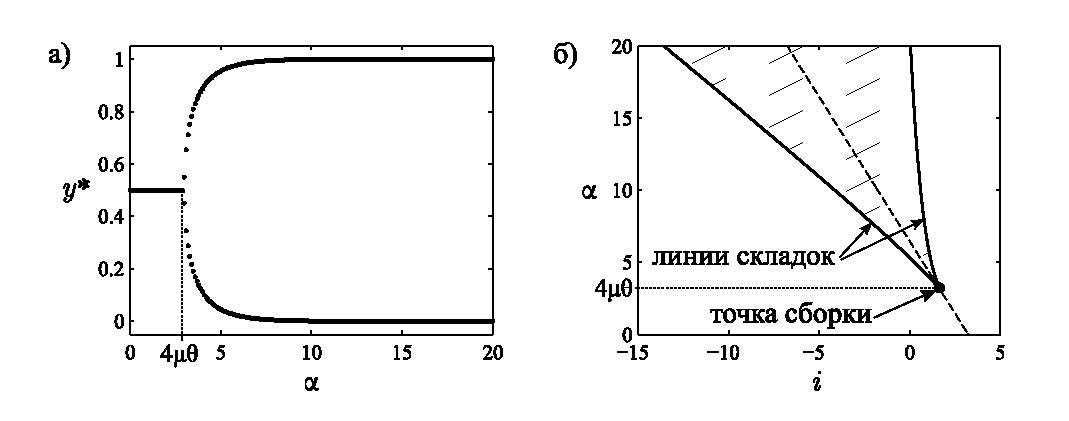
\includegraphics[width=1.0\textwidth]{analysis_sigm_bifurcations}}
    \makebox[\textwidth][c]{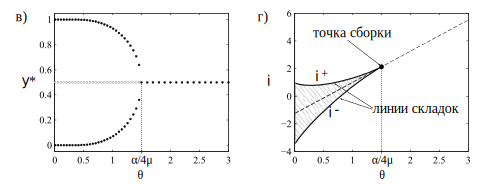
\includegraphics[width=1.0\textwidth]{analysis_sigm_bifurcations_p2}}
    \caption{Бифуркационные диаграммы: а,в) бифуркации типа суперкритическая \inquotes{вилка} (точки устойчивого равновесия отмечены закрашенными кругами, неустойчивого -- проколотыми); б,г) бифуркации типа \inquotes{сборка} (би-стабильная область заштрихована, уни-стабильная -- нет).}
    \label{fig:analysis_sigm_bifurcations}
\end{figure}

Как было замечено ранее (\seefigure~\ref{fig:analysis_sigm_equilibriums}б), при наличии $s$-образной складки в графике функции $F(\scalar{y})$ система~\eqref{eq:simple_microensemble_model} в зависимости от значения параметра $i$ может иметь одно или два устойчивых решения. С учётом найденных точек экстремума $\scalar{y}^{\mp}$~\eqref{eq:sigm_stability_bounds_y}, бифуркационной точки параметра $\alpha$~\eqref{eq:sigm_bifurcation_alpha} и выражения~\eqref{eq:graphic_solution}, которое определяет связь между переменными $\scalar{y}$ и $\scalar{i}$ для точек равновесия, область существования двух устойчивых состояний модели будет определяться следующим образом:
\begin{equation}
    \nonumber
    \left\{(\alpha, \scalar{i}) \mid \alpha > 4 \mu \theta, i^{-} < \scalar{i} < i^{+}\right\},
\end{equation}
где:
\begin{equation}
    \label{eq:sigm_stability_bounds_i}
    i^{\mp} = -\alpha \scalar{y}^{\mp} + \mu \theta g_{\sigma}(\scalar{y}^{\mp}).
\end{equation}

Данная ситуация соответствует бифуркации типа \inquotes{сборка}, что продемонстрировано \onfigure~\ref{fig:analysis_sigm_bifurcations}б: при фиксированном значении параметра $\alpha$, допускающем существование би-стабильного режима, монотонное возрастание значения параметра $i$ приводит к тому, что в точке $i^{-}$ единственная точка устойчивого равновесия дополняется парой из точек неустойчивого и устойчивого равновесия (\onfigure~\ref{fig:analysis_sigm_equilibriums}в точки $\scalar{y}^{*}_{2}$, $\scalar{y}^{*}_{3}$ и $\scalar{y}^{*}_{1}$ соответственно), а в точке $i^{+}$ изначально существовавшая точка устойчивого равновесия аннигилируется вместе с точкой неустойчивого равновесия, в результате чего в системе вновь останется единственное и при том устойчивое решение. 

Рассмотренное изображением является проекцией $s$-образной складки, возникающей на поверхности решений системы~\eqref{eq:simple_microensemble_model} --- сама поверхность изображена \onfigure~\ref{fig:analysis_sigm_solution_surface}а. Так же для наглядности \onfigure~\ref{fig:model_sigm_configurations_by_alpha} показаны различные срезы этой поверхности, привязанные к плоскости параметров. При этом бифуркационная точка, называемая точкой сборки, задаёт в плоскости параметров место возникновения складки и определяется равенством~\eqref{eq:sigm_bifurcation_alpha} и выражением~\eqref{eq:sigm_stability_bounds_i} как:
\begin{equation}
    \nonumber
    (\alpha, \scalar{i}) = (4 \mu \theta, \mu \theta).
\end{equation}

\begin{figure}[t]
    \makebox[\textwidth][c]{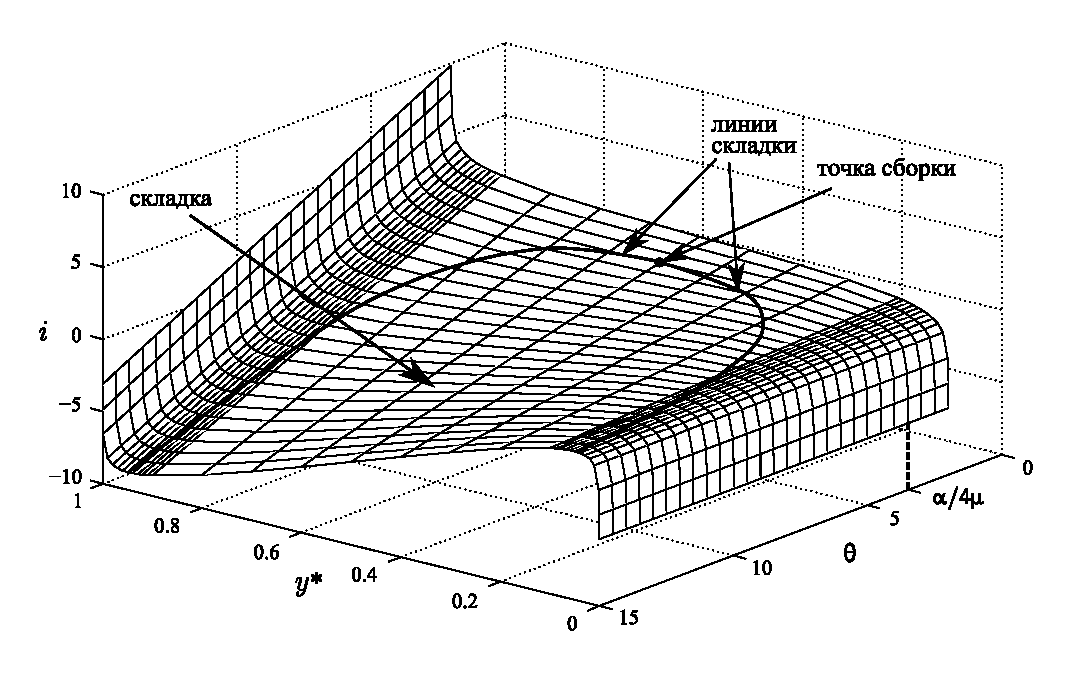
\includegraphics[width=0.95\textwidth]{analysis_sigm_solution_surface}}
    \makebox[\textwidth][c]{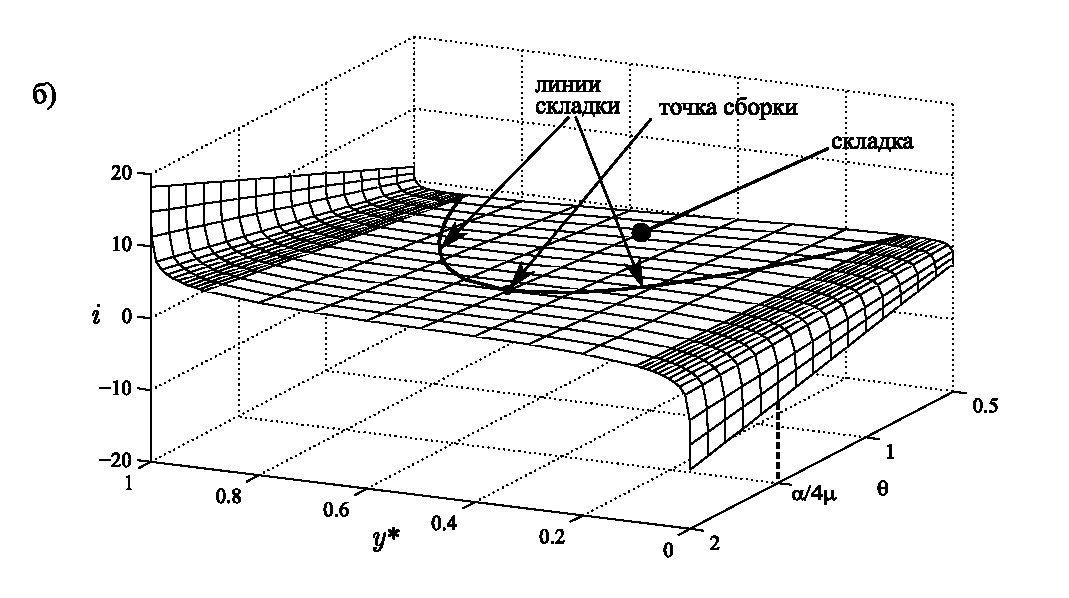
\includegraphics[width=0.95\textwidth]{analysis_sigm_solution_surface_p2}}
    \caption{Поверхность решений системы~\eqref{eq:simple_microensemble_model}, построенная вариацией параметров: а) $\alpha$ и $\scalar{i}$ при $\theta = 1, \mu = 0,75$; б) $\theta$ и $\scalar{i}$ при $\alpha = 4,5, \mu = 0,75$.}
    \label{fig:analysis_sigm_solution_surface}
\end{figure}

Как отмечалось выше, в выражение~\eqref{eq:sigm_stability_bounds_y}, определяющее точки экстремума кривой решений $F(y)$, параметр $\theta$ входит обратно пропорционально параметру $\alpha$, поэтому справедливо ожидать, что бифуркационный анализ относительно параметра $\theta$ даст аналогичные полученным для параметра $\alpha$ результаты.

Бифуркация типа суперкритическая \inquotes{вилка} продемонстрирована \onfigure~\ref{fig:analysis_sigm_bifurcations}в: при монотонном возрастании значения параметра $\theta$ две точки устойчивого равновесия сливаются вместе с точкой неустойчивого равновесия, образуя при этом одну устойчивую точку (\onfigure~\ref{fig:analysis_sigm_bifurcations}г пунктиром обозначены соответствующие при этом значения параметра $i$, обеспечивающие симметрию \inquotes{вилки}). Точка бифуркации находится из тех же соображений, что и бифуркационная точка~\eqref{eq:sigm_bifurcation_alpha}:
\begin{equation}
    \label{eq:sigm_bifurcation_theta}
    \theta =  \alpha / 4 \mu.
\end{equation}

Бифуркация типа \inquotes{сборка} изображена \onfigure~\ref{fig:analysis_sigm_bifurcations}г: когда значение параметра $\theta$ фиксированно и допускает существование би-стабильного режима, прохождение точек $i^{-}$ и $i^{+}$ при возрастании значения параметра $\scalar{i}$ приводит, соответственно, сначала к появлению дополнительной точки устойчивого равновесия, а затем к аннигиляции изначальной точки устойчивого равновесия. При этом область существования двух устойчивых состояний модели можно определить как множество: 
\begin{equation}
    \nonumber
    \left\{(\theta, \scalar{i}) \mid \theta < \alpha / 4 \mu, i^{-} < \scalar{i} < i^{+}\right\}.
\end{equation}

Поверхность решений системы~\eqref{eq:simple_microensemble_model} для данного случая продемонстрированна \onfigure~\ref{fig:analysis_sigm_solution_surface}б, где отмечено наличие $s$-образной складки, а срезы этой поверхности, привязанные к плоскости параметров, изображены \onfigure~\ref{fig:model_sigm_configurations_by_theta}. При этом точка сборки, исходя из равенства~\eqref{eq:sigm_bifurcation_theta} и выражения~\eqref{eq:sigm_stability_bounds_i}, будет равна:
\begin{equation}
    \nonumber
    (\theta, \scalar{i}) = (\alpha / 4 \mu, \alpha / 4).
\end{equation}

Если объединить результаты, полученные для параметров $\alpha$ и $\theta$, то область существования двух устойчивых решений системы~\eqref{eq:simple_microensemble_model}, как следует из выражений~\eqref{eq:sigm_bifurcation_alpha} и~\eqref{eq:sigm_bifurcation_theta}, будет определяться в пространстве этих параметров условием $\alpha \big/ \theta > 4 \mu$. Само пространство изображено \onfigure~\ref{fig:analysis_sigm_alpha_vs_theta}, где области моно- и би-стабильности отвечают соответственно верхней и нижней полуплоскостям, которые разделены прямой с коэффициентом наклона $1 \big/ 4 \mu$.

\IncludeFigure[ht]{analysis_sigm_alpha_vs_theta}{Области моно- и би-стабильности системы~\eqref{eq:simple_microensemble_model} на плоскости параметров $\alpha$ и $\theta$ (закрашены без и со штриховкой соотвественно).}

Однако стоит отметить, что данное условие является необходимым, но не достаточным для наличия двух устойчивых точек в модели --- как отмечалось выше при выводе величин $i^{\mp}$~\eqref{eq:sigm_stability_bounds_i}, значение параметра $\scalar{i}$ должно при этом лежать в интервале значений $\left(i^{-}; i^{+}\right)$. Таким образом, область би-стабильности будет определяться как множество:
\begin{equation}
    \nonumber
    \left\{(\alpha, \theta, \scalar{i}) \mid \alpha \big/ \theta > 4 \mu, i^{-} < \scalar{i} < i^{+}\right\}.
\end{equation}

\subsubsection{Дополнительные замечания}

Согласно выражению~\eqref{eq:sigm_stability_bounds_y} параметры $\alpha$ и $\theta$ вносят пропорциональный вклад в значения точек экстремума $y^{-}$ и $y^{+}$, однако их влияние на значения бифуркационных величин $i^{+}$ и $i^{-}$ имеет более сложный характер, что графически изображено \onfigure~\ref{fig:analysis_sigm_params_dependency}, а так же можно наблюдать \onfigure~\ref{fig:analysis_sigm_bifurcations}б,г.
\IncludeFigure[ht]{analysis_sigm_params_dependency}{Зависящие от параметров $\alpha$ и $\theta$ поверхности точек бифуркации $i^{-}$ и $i^{+}$, проекции которых на плоскости $\left(\alpha,\scalar{i}\right)$ и $\left(\theta,\scalar{i}\right)$ изображены \onfigure~\ref{fig:analysis_sigm_bifurcations}б,г.}

Для того, чтобы оценить это влияние, представим, что точки $i^{-}$ и $i^{+}$ определяются соответствующими параметрическими функциями $i^{-}(z)$ и $i^{+}(z)$ с параметром $z \in \left[z_{0}; z_{1}\right]$. Зададим эти функции, исходя из определения самих величин $i^{\mp}$~\eqref{eq:sigm_stability_bounds_i}, подставив в него выражение для корней $y^{\mp}$~\eqref{eq:sigm_stability_bounds_y} и определение обратной функции активации $g_{\sigma}$~\eqref{eq:unactivation_function_sigma}:
\begin{equation}
    \nonumber
    i^{\mp}(z) = \alpha \left(-(0,5 \pm 0,5z) + \left(0,25 - 0,25z^2\right) \left(3 + \ln\left(\dfrac{1 \pm z}{1 \mp z}\right)\right)\right),
\end{equation}
где $z(\theta) = 2 \sqrt{0,25 - \mu\theta/\alpha}$, причём $z \in \left(0;1\right)$ при $\theta \in \left(\alpha/4\mu;0\right)$. Далее, применяя к функции логарифма разложение в ряд Тейлора в окрестности нуля, мы получим следующее выражение:
\begin{equation}
    \nonumber
    \begin{aligned}
        i^{\mp}(z) &= \alpha \left( -(0,5 \pm 0,5z) + \left(0,25 - 0,25z^2\right) \left(3 \pm 2\sum_{n=0}^{\infty}\dfrac{z^{2n+1}}{2n+1}\right) \right) = \\
        &= 0,25 \alpha \left( 1 \mp 2z - 3z^2 \pm 2 \left(1 - z^2\right) \sum_{n=0}^{\infty}\dfrac{z^{2n+1}}{2n+1} \right) = \\
        &= 0,25 \alpha \left( 1 \mp 2z - 3z^2 \pm 2\left(z + \sum_{n=1}^{\infty}\dfrac{z^{2n+1}}{2n+1} - \sum_{n=0}^{\infty}\dfrac{z^{2n+3}}{2n+1}\right)\ \right).
    \end{aligned}
\end{equation}
После перенумерации первой суммы так, чтобы индекс начинался с нуля, и сложения коэффициентов при одинаковых степенях получим окончательное выражение в виде:
\begin{equation}
    \label{eq:sigm_approximation_i}
    i^{\mp}(z) = 0,25 \alpha \left( 1 - 3z^2 \mp 4 \sum_{n=0}^{\infty}\dfrac{z^{2n+3}}{(2n+3)(2n+1)} \right),
\end{equation}
откуда можно сделать вывод, что значения параметрических кривых, а значит и значения величин $i^{\pm}$, на границах области определения зависят исключительно от параметра $\alpha$, причём:
\begin{equation}
    \nonumber
    \begin{cases}
        \lim_{\theta \to +0} i^{+} &= 0 \\
        \lim_{\theta \to +0} i^{-} &= -\alpha 
    \end{cases}
    \quad \text{ и } \quad
    \begin{cases}
        \lim_{\theta \to \sfrac{\alpha}{4\mu} - 0} i^{+} &= \alpha / 4 \\
        \lim_{\theta \to \sfrac{\alpha}{4\mu} - 0} i^{-} &= \alpha / 4
    \end{cases}.
\end{equation}

С учётом нашего предположения о том, что параметра $\alpha$, как и параметр $\mu$, фиксируется и не меняется в процессе функционирования модели, получается, что параметр $\alpha$ задаёт точный вид параметрических кривых $i^{\pm}(z(\theta))$, в то время как параметр $\theta$ влияет только на выбор конкретных точек на этих кривых.

%которое позволяет оценить характер изменения величин $i^{-}$ и $i^{+}$, а так же позволяет определить монотонность убывания величины $\Delta i(z) = i^{+}(z) - i^{-}(z)$ при возрастании значении $\theta$.

%==============================================================================
\subsection{Модель с оригинальной функцией активации}  \label{subsection:analysis_origin}

Теперь рассмотрим вариант модели с использованием \textit{оригинальной} функции активации (\acr{OAF}-модель). На рисунке~\ref{fig:analysis_origin_equilibriums} приведены графические решения системы~\eqref{eq:simple_microensemble_model} согласно выражению~\eqref{eq:graphic_solution} и соответствующие графики функции $F(\scalar{y})$ для следующих наборов значений параметров: а) $\alpha = 0  $ и $i = 2$; б) $\alpha = 0,5$ и $i = 0,95$; в) $\alpha = 2,5$ и $i = 2$; г) $\alpha = 5,5$ и $i = 0,5$; д) $\alpha = 60$ и $i = -20$, где значения  $\mu = 0,75$, $\theta = 1$ и $p = 1,0$ одинаковы для всех вариантов. Сразу заметим, учитывая результаты анализа из~\autoref{subsection:analysis_sigm}, что основные отличия от \acr{SAF}-модели будут следствием наличия не одной, а двух $s$-образных складок в графике решений, которые дают большее разнообразие режимов функционирования (\seefigure~\ref{fig:analysis_origin_equilibriums}):
\IncludeFigure[p]{analysis_origin_equilibriums}{Графическое решение системы~\eqref{eq:simple_microensemble_model} и график функции $F(\scalar{y})$ для случаев: а) отсутствия складок; б) наличия только $low$-складки; в) наличия двух, но неперекрывающихся складок; г) наличия двух, но перекрывающихся складок; д) наличия слившихся складок.}
\begin{itemize}
    \item[а)] Система имеет ровно одну точку устойчивого равновесия (точка $y^{*}$), которая полностью определяется параметрами системы.
    \item[б)] Система может иметь одну (не показана на рисунке) или две точки устойчивого равновесия (точки $y^{*}_{1,3}$), где область би-стабильности определяется положением первой складки (далее, $low$-складка), \ie интервалом $\scalar{i} \in (i_{low}^{-}; i_{low}^{+})$.
    \item[в)] Система вновь может иметь одну (не показана на рисунке) или две точки устойчивого равновесия (точки $y^{*}_{1,3}$), однако область би-стабильности, помимо положения $low$-складки, определяется так же положением второй складки (далее, $high$-складка), \ie определяется интервалом $\scalar{i} \in (i_{low}^{-}; i_{low}^{+}) \cup (i_{high}^{-}; i_{high}^{+})$.
    \item[г)] Система может иметь одну, две (не показаны на рисунке) или три точки устойчивого равновесия (точки $y^{*}_{1,3,5}$). При этом область би-стабильности, как и ранее, определяется положением $low$- и $high$-складок, за исключением области их пересечения --- интервала $\scalar{i} \in (i_{low}^{-}; i_{low}^{+}) \cap (i_{high}^{-}; i_{high}^{+})$, который соответствует области три-стабильности системы.
    \item[д)] Система вновь может иметь одну (не показана на рисунке) или две точки устойчивого равновесия (точки $y^{*}_{1,3}$), однако область би-стабильности определяется положением складки, возникшей в результате слияния $low$- и $high$-складок (далее, $broad$-складка), \ie определяется интервалом $\scalar{i} \in (i_{high}^{-}; i_{high}^{+})$.
\end{itemize}

\subsubsection{Анализ устойчивости точек равновесия}

Как и в~\autoref{subsection:analysis_sigm}, для определения интервалов устойчивости-неустойчивости точек равновесия $\scalar{y}^{*}$ необходимо решить равенство $F^{\prime}(\scalar{y}) = 0$, которое в соответствии с определением функции $g_{s}$~\eqref{eq:unactivation_function_original} примет вид:
\begin{equation}
\nonumber
    F^{\prime}(\scalar{y}) = \dfrac{d}{d\scalar{y}}\left( \alpha \scalar{y} + \scalar{i} - \mu \theta g(\scalar{y}) \right) = 
    \begin{cases}
        \alpha - \dfrac{312 \mu \theta \scalar{x}}{(\scalar{x} + 1)^{2}} = 0,   & \scalar{x} \in \left(x_{01}; x_{12}\right] \\
        \alpha - \dfrac{z_{12} \mu \theta}{(\scalar{y} - 1)^{2}} = 0,           & \scalar{y} \in \left(y_{12}; 1\right] \\
    \end{cases}
\end{equation}
где $\scalar{x} = e^{-120 \cdot (\scalar{y} - 0,1935)}$, а $x_{01} = e^{120 \cdot 0,1935}$ и $x_{12} = e^{-120 \cdot (y_{12} - 0,1935)}$ (приближённо, $x_{01} \approx 1,2 \cdot 10^{10}$ и $x_{12} \approx 2,1 \cdot 10^{-3}$). Соответственно, обратное преобразование будет определено как $\scalar{y} = 0,1935 - \ln(\scalar{x}) / 120$.

Сразу отметим, что исходя из определения функции $g_{s}$ в точке $\scalar{y} = 0$, $F^{\prime}(0) = -\infty$ и поэтому точка равновесия $\scalar{y}^{*} = 0$ всегда устойчива и существует при $\scalar{i} < \mu \theta u_{01}$ --- обозначим это решение как $y_{low}^{+}$.

Для решения же полученных равенств в выражении $F^{\prime}(\scalar{y})$ приведём их к виду квадратных уравнений. Для этого, во-первых, примем во внимание, что переменная $\scalar{y}$ в системе~\eqref{eq:simple_microensemble_model} достигает значения 1 лишь в пределе, что обусловлено свойством \textit{оригинальной} функции активации: $\scalar{y} = \lim_{\scalar{x} \to \infty} f(\scalar{x}) = 1$. Во-вторых, отметим, что при $\alpha = 0$ решений не существует и $F^{\prime}(\scalar{y}) < 0\ \forall \scalar{y}$ --- однако это условие в дальнейшем войдёт в более общее условие устойчивости, поэтому отдельно мы его рассматривать не будет. Таким образом, после деления равенств на $\alpha$ и домножения, соответственно, на $(\scalar{x} + 1)^{2}$ и $(\scalar{y} - 1)^{2}$ мы получим следующие квадратные уравнения:
\begin{equation}
    \nonumber
    \begin{cases}
        \scalar{x}^{2} + \left( 2 - 312 \mu \theta / \alpha \right) \scalar{x} + 1 = 0,     & \scalar{x} \in \left(x_{01}; x_{12}\right]    \\
        \scalar{y}^{2} - 2 \scalar{y} + \left( 1 - z_{12} \mu \theta / \alpha \right) = 0,  & \scalar{y} \in \left(y_{12}; 1\right]         \\
    \end{cases}
\end{equation}
решением которых будут корни:
\begin{equation}
    \nonumber
    \begin{cases}
        \scalar{x}_{1,2}    &= \left( 156 \mu \theta / \alpha - 1\right) \pm \sqrt{\left( 156 \mu \theta / \alpha - 1\right)^{2} - 1},      \\
        \scalar{y}_{3}      &= 1 - \sqrt{z_{12} \mu \theta / \alpha},                                                                       \\
    \end{cases}
\end{equation}
а корень $\scalar{y}_{4} = 1 + \sqrt{z_{12} \mu \theta / \alpha}$ не рассматривается, т.к. при любых допустимых значениях параметров $\scalar{y}_{4} > 1$, \ie его значение лежит вне области определения переменной $\scalar{y}$.

Для дальнейшего удобства обозначим корни следующим образом:
\begin{equation}
    \begin{cases}
        \label{eq:origin_stability_bounds_y}
        \scalar{y}^{-}_{low}    &= 0,1935 - \dfrac{1}{120} \ln\left( \left( 156 \mu \theta / \alpha - 1\right) + \sqrt{\left( 156 \mu \theta / \alpha - 1\right)^{2} - 1} \right), \\
        \scalar{y}^{+}_{high}   &= 0,1935 - \dfrac{1}{120} \ln\left( \left( 156 \mu \theta / \alpha - 1\right) - \sqrt{\left( 156 \mu \theta / \alpha - 1\right)^{2} - 1} \right), \\
        \scalar{y}^{-}_{high}   &= 1 - \sqrt{z_{12} \mu \theta / \alpha}, \\
    \end{cases}
\end{equation}
предполагая, что величины $\scalar{y}^{-}_{low}$ и $\scalar{y}^{+}_{high}$ являются вещественными числами, \ie точками, где функция $F^{\prime}(\scalar{y})$ обращается в ноль. Непосредственно из уравнений следует, что для корня $\scalar{y}^{-}_{high}$ область допустимых значений определяется интервалом $\left(y_{12}; 1\right]$, а для корней $\scalar{y}^{-}_{low}$ и $\scalar{y}^{+}_{high}$ --- интервалом $\left(0; y_{12}\right]$. Кроме того, как следует из Приложения~\ref{appendix:origin_roots_existance} \inquotes{\nameref{appendix:origin_roots_existance}}, область существования корней в пространстве параметров модели будет определяться, исходя из следующих условий:
\begin{itemize}
    \item $1 / 78 < \mu \theta / \alpha < (x_{01} + 1)^{2} / (312 x_{01})$ для корня $\scalar{y}^{-}_{low}$, причём на левой границе $\scalar{y}^{-}_{low} = 0,1935$, а на правой -- $\scalar{y}^{-}_{low} = 0$;
    \item $1 / 78 < \mu \theta / \alpha < (x_{12} + 1)^{2} / (312 x_{12})$ для корня $\scalar{y}^{+}_{high}$, причём на левой границе $\scalar{y}^{+}_{high} = 0,1935$, а на правой -- $\scalar{y}^{+}_{high} = y_{12}$;
    \item $\mu \theta / \alpha < \left(1 - y_{12}\right)^{2} / z_{12}$ для корня $\scalar{y}^{-}_{high}$, причём на границе значение $\scalar{y}^{-}_{high} = y_{12}$.
\end{itemize}

Отметим, что доказательство включения или выключения в интервалы устойчивости граничных точек, где $F^{\prime}(\scalar{y}) = 0$, основывается на том же принципе, что и в аналогичном подразделе~\autoref{subsection:analysis_sigm}, а именно на анализе значений производной в окрестности этих точек. В виду очевидности данного принципа мы будем сразу учитывать его в результатах без его явного применения к каждой из интересующих нас точек. Таким образом, обозначив через $D = \left( 156 \mu \theta / \alpha - 1\right)^{2} - 1$, мы получим следующее:
\begin{enumerate}[wide]
    \item Если $D < 0$, то корни $\scalar{y}^{-}_{low}$ и $\scalar{y}^{+}_{high}$ не определены и, как показано \onfigure~\ref{fig:analysis_origin_stability}в, $\forall\scalar{y} \in \left(0; y_{12}\right]\ F^{\prime}(\scalar{y}) > 0$. Кроме того, в этом случае $\mu \theta / \alpha < 1 / 78$ и, как следствие, $y_{high}^{-} \in (1 - \sqrt{z_{12} / 78}; 1] \subset (y_{12}; 1]$, \ie всегда лежит в области допустимых значений. Поэтому область устойчивых решений модели будет определяться множеством точек $\{0\} \cup (y_{high}^{-}; 1]$, на котором $F^{\prime}(\scalar{y}) < 0$.
    \item Если $D = 0$, то корни $\scalar{y}^{-}_{low}$ и $\scalar{y}^{+}_{high}$ будут равны константе $y^{\sim} = 0,1935$ и, как результат, $\forall\scalar{y} \in \left(0; y_{12}\right]\ F^{\prime}(\scalar{y}) \ge 0$, где равенство достигается при $y = y^{\sim}$. А в виду того, что решение $y^{*} = y^{\sim}$ неустойчиво, область устойчивых решений модели будет такой же, что и в случае, когда $D < 0$, \ie $\{0\} \cup (y_{high}^{-}; 1]$.
    \item Если $D > 0$, то все корни будут различными вещественными числами и в этом случае необходимо учитывать области их существования в пространстве параметров модели. Заметим, что правые границы областей существования корней $\scalar{y}^{\pm}_{high}$ совпадают по значению и включены в соответствующую облать существования корня $\scalar{y}^{-}_{low}$, поэтому область устойчивых решений модели, где $F^{\prime}(\scalar{y}) < 0$, будет определяться или интервалом $[0; 1]$ (\seefigure~\ref{fig:analysis_origin_stability}а), или множеством $\{0\} \cup (y_{low}^{-}; 1]$, или множеством $\{0\} \cup (y_{low}^{-}; y_{high}^{+}) \cup (y_{high}^{-}; 1]$ (\seefigure~\ref{fig:analysis_origin_stability}б).
\end{enumerate}

\IncludeFigure[t]{analysis_origin_stability}{Определяемые знаком функции $F^{\prime}(\scalar{y})$ интервалы устойчивых решений системы~\eqref{eq:simple_microensemble_model} в режимах: а)~моностабильности; б)~три-стабильности; в)~би-стабильности (участки графика функции $F$ с устойчивыми и неустойчивыми решениями обозначены соответственно сплошной и пунктирной линиями).}

Как видно, области существования устойчивых решений системы~\eqref{eq:simple_microensemble_model} в пространстве параметров модели определяются как значением величины $D$, так и граничными условиями, связанными с кусочно-заданным видом \textit{оригинальной} функции активации. Получить представление об этих областях можно \onfigure~\ref{fig:analysis_origin_equilibrium_areas}, где изображены спроецированные на соответствующие плоскости границы $\scalar{y}_{low}^{\pm}$ и $\scalar{y}_{high}^{\pm}$ относительно значений: а)~параметра $\alpha$ при $\theta = 1$ и $\mu = 0,75$; б)~параметра $\theta$ при $\alpha = 3,5$ и $\mu = 0,75$. Видно наличие более сложной структуры этих областей по сравнению с \acr{SAF}-моделью (\seefigure~\ref{fig:analysis_sigm_equilibrium_areas}). 
%Кроме того можно отметить, что область $(y_{low}^{-}; y_{low}^{+}) \subset (0; 0,245)$ существует 

\IncludeFigure[t]{analysis_origin_equilibrium_areas}{Зависимость областей существования устойчивых (без штриховки) и неустойчивых (с диагональной штриховкой) решений системы~\eqref{eq:simple_microensemble_model} относительно значений: а)~параметра $\alpha$; б)~параметра $\theta$.} 

\subsubsection{Бифуркационный анализ}

Аналогично~\autoref{subsection:analysis_sigm}, для определения критических значений параметров, при которых происходят качественные изменения в характере функционирования модели, необходимо проанализировать пространство параметров модели с точки зрения бифуркационного анализа. Как и ранее, в первую очередь мы рассмотрим параметр $\alpha$, а затем -- параметр $\theta$.

Как показано \onfigure~\ref{fig:analysis_origin_bifurcations}а, по сравнению с \acr{SAF}-моделью (\seefigure~\ref{fig:analysis_sigm_bifurcations}а) здесь наблюдается целая серия бифуркаций типа суперкритическая \inquotes{вилка} (\onfigure~\ref{fig:analysis_origin_bifurcations}б пунктиром обозначены соответствующие значения параметра $\scalar{i}$, обеспечивающие форму изображённой \inquotes{вилки}): при монотонном возрастании значения параметра $\alpha$ сначала дважды наблюдается эффект возникновения дополнительной пары точек устойчивого и неустойчивого равновесия, а затем происходит аннигиляция одной из пар и, как результат, остаётся только две устойчивые точки, такие что: $\scalar{y}^{*}_{1} = 0$ и $\lim_{\alpha \to \inf} \scalar{y}^{*}_{2} = 1$. Как отмечалось в~\autoref{subsection:analysis_sigm}, в основе данной бифуркации лежит явление возникновения (или исчезновения) $s$-образных складок в кривой решений $F(\scalar{y})$ за счёт по возникновения (или исчезновения) точек локального экстремума. В данном случае эти точки определяются корнями $\scalar{y}^{-}_{low}$ и $\scalar{y}^{\pm}_{high}$~\eqref{eq:origin_stability_bounds_y} и, исходя из условий их существования в пространстве параметров, мы можем определить три точки бифуркации:
\begin{figure}[t]
    \makebox[\textwidth][c]{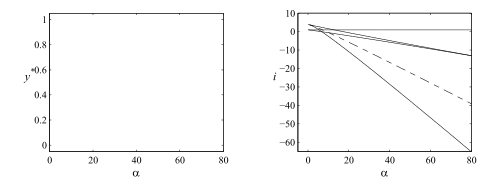
\includegraphics[width=1.0\textwidth]{analysis_origin_bifurcations}}
    \makebox[\textwidth][c]{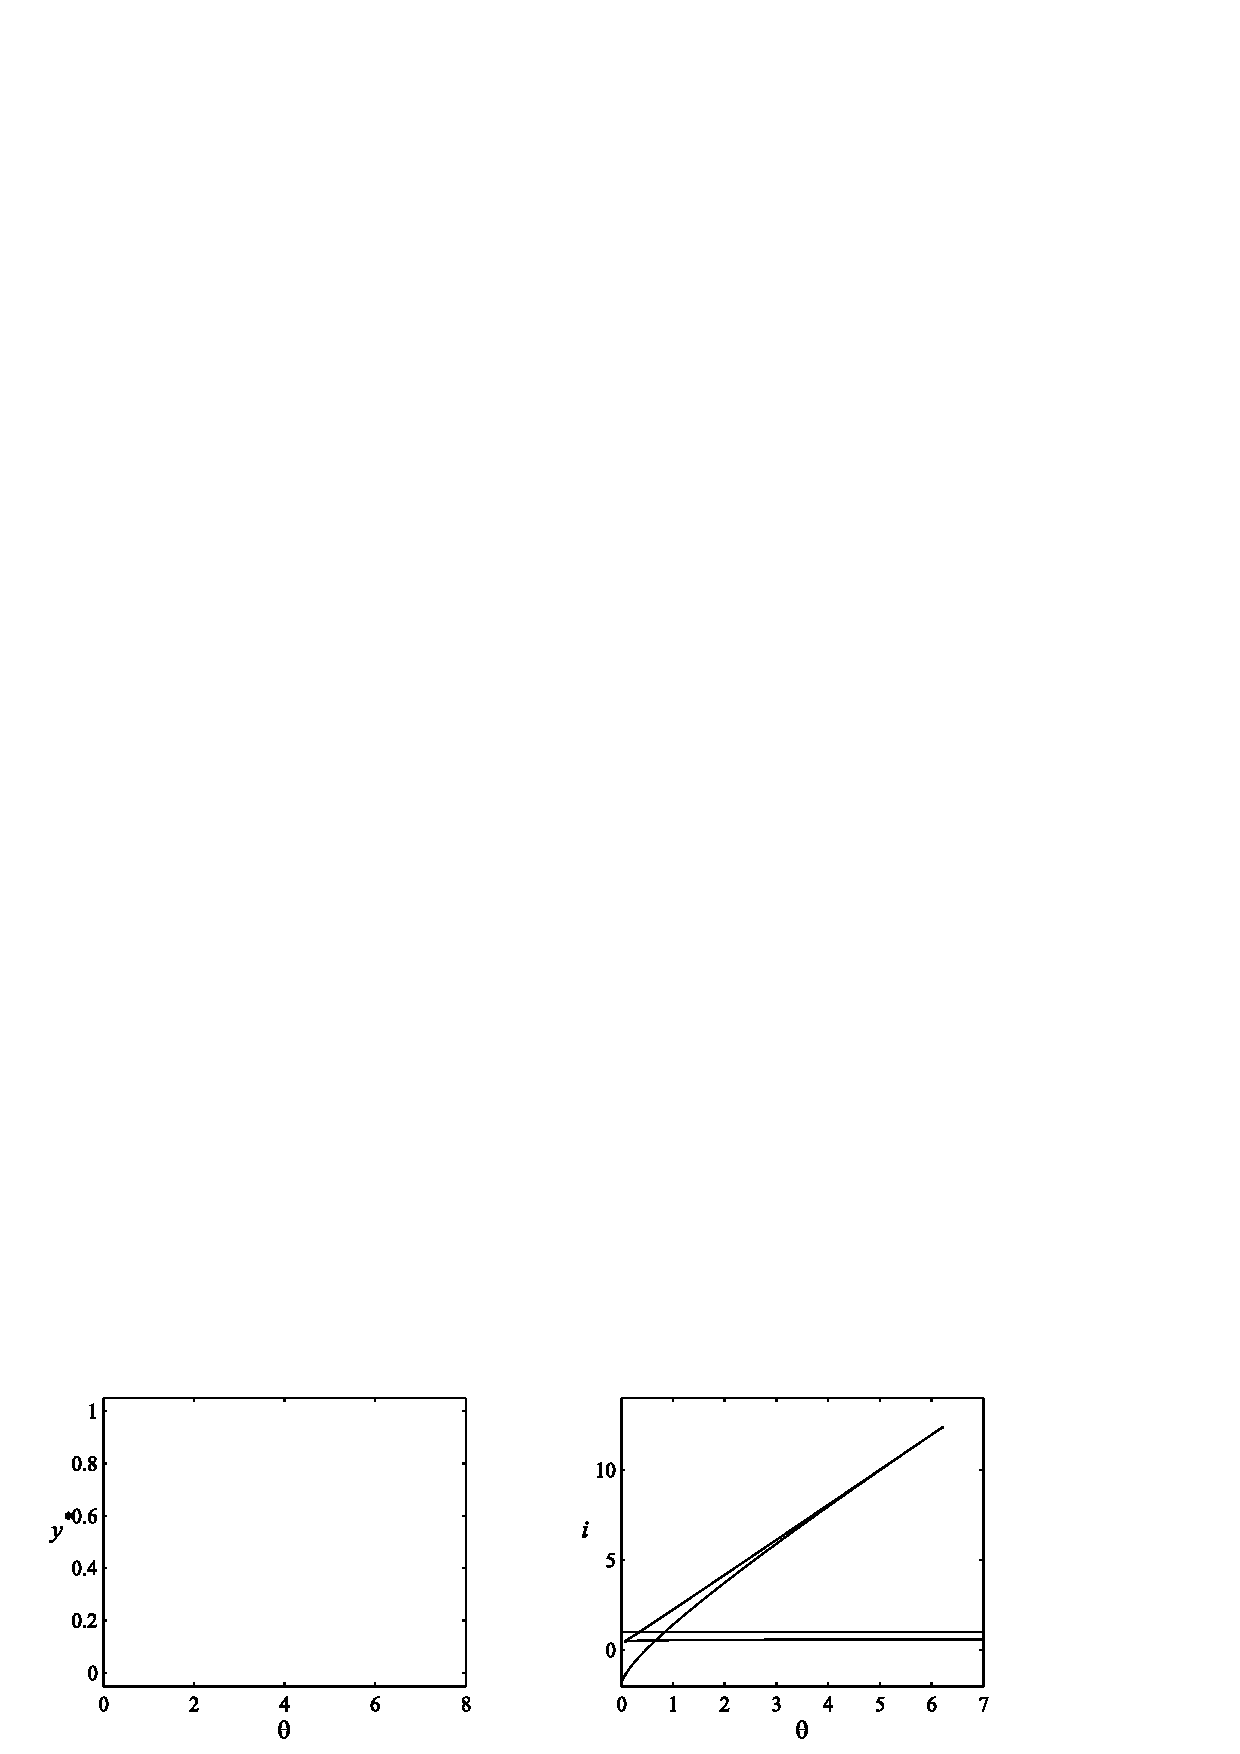
\includegraphics[width=1.0\textwidth]{analysis_origin_bifurcations_p2}}
    \caption{Бифуркационные диаграммы: а,в) бифуркации типа суперкритическая \inquotes{вилка} (точки устойчивого равновесия отмечены закрашенными кругами, неустойчивого -- проколотыми); б,г) бифуркации типа \inquotes{сборка} (три-стабильная область закрашена двойной штриховкой, би-стабильная -- диагональной, уни-стабильная -- без штриховки).}
    \label{fig:analysis_origin_bifurcations}
\end{figure}
\begin{equation}
    \label{eq:origin_bifurcation_alpha}
    \begin{aligned}
        % переобозвать  альфы как high/low^+/-
        \alpha_{1} &= \dfrac{312 x_{01}}{(x_{01} + 1)^2} \cdot \mu \theta \approx 2,6 \cdot 10^{-8} \cdot \mu \theta, \\
        \alpha_{2} &= \dfrac{z_{12}}{(1 - y_{12})^2} \cdot \mu \theta \approx 6,4 \cdot 10^{-1} \cdot \mu \theta, \\
        \alpha_{3} &= 78 \cdot \mu \theta, 
    \end{aligned}
\end{equation}
где значения $\alpha_{1,2}$ соответствуют точкам появления $low$- и $high$-складок, когда возникают дополнительные точки устойчивого равновесия, а значение $\alpha_{3}$ --- точке слияния этих складок в $broad$-складку, когда одна из точек устойчивого равновесия исчезает. Стоит отметить, что для определения значения $\alpha_{2}$ было использовано граничное условие существования корня $\scalar{y}^{-}_{high}$, хотя вместо него можно было бы использовать соответствующее граничное условие существования корня $\scalar{y}^{+}_{high}$ в виду того, что эти корни возникают одновременно как пара точек, определяющая положение $high$-складки, и поэтому соответствующие границы совпадают, что так же легко проверяется непосредственными вычислениями.

При рассмотрении модели на плоскости параметров $\alpha$ и $\scalar{i}$ будет наблюдаться бифуркация типа \inquotes{сборка}, как показано \onfigure~\ref{fig:analysis_origin_bifurcations}б: при значениях параметра $\alpha$, которые допускают мульти-стабильность модели, будет ли система~\eqref{eq:simple_microensemble_model} иметь одно или несколько устойчивых решений зависит от значения параметра $\scalar{i}$. А с учётом найденных точек экстремума $\scalar{y}^{\mp}_{low}$ и $\scalar{y}^{\mp}_{high}$~\eqref{eq:origin_stability_bounds_y}, бифуркационных точек параметра $\alpha$~\eqref{eq:origin_bifurcation_alpha}, а так же выражения~\eqref{eq:graphic_solution}, которое задаёт связь между переменными $\scalar{y}$ и $\scalar{i}$ для устойчивых решений, область существования не менее двух устойчивых состояний модели будет определяться объединением следующих множеств:
\begin{equation}
    \label{eq:origin_stability_area}
    \begin{aligned}
        &\{ (\alpha, \scalar{i}) \mid \alpha_{1} < \alpha < \alpha_{3}, i^{-}_{low} < \scalar{i} < i^{+}_{low} \}, \\
        &\{ (\alpha, \scalar{i}) \mid \alpha_{2} < \alpha < \alpha_{3}, i^{-}_{high} < \scalar{i} < i^{+}_{high} \}, \\
        &\{ (\alpha, \scalar{i}) \mid \alpha \ge \alpha_{3}, i^{-}_{high} < \scalar{i} < i^{+}_{low} \}, \\
    \end{aligned}
\end{equation}
где:
\begin{equation}
    \label{eq:origin_stability_bounds_i}
    i^{\mp}_{low/high} = -\alpha \scalar{y}^{\mp}_{low/high} + \mu \theta g_{s}(\scalar{y}^{\mp}_{low/high}).
\end{equation}

Эти множества являются проекциями соответственно $low$-, $high$- и $broad$-складок, которые возникают на поверхности решений системы~\eqref{eq:simple_microensemble_model} --- сама поверхность изображена \onfigure~\ref{fig:analysis_origin_solution_surface}а. Для наглядности \onfigure~\ref{fig:model_origin_configurations_by_alpha} так же показаны различные срезы этой поверхности, привязанные к плоскости параметров. При этом точки сборки, как следует из найденных бифуркационных точек параметра $\alpha$~\eqref{eq:origin_bifurcation_alpha} и выражения~\eqref{eq:origin_stability_bounds_i}, определяются как:
\begin{equation}
    \nonumber
    \begin{aligned}
        &(\alpha, \scalar{i}) = \left( \dfrac{312 x_{01}}{(x_{01} + 1)^2} \cdot \mu \theta ,\ u_{01} \cdot \mu \theta \right), \\
        &(\alpha, \scalar{i}) = \left( \dfrac{z_{12}}{(1 - y_{12})^2} \cdot \mu \theta     ,\ \minus \dfrac{z_{12} y_{12}}{(1 - y_{12})^2} \cdot \mu \theta + u_{12} \cdot \mu \theta \right) , \\
        &(\alpha, \scalar{i}) = \left( 78 \cdot \mu \theta,\ \minus 13,793 \cdot \mu \theta \right) .
    \end{aligned}
\end{equation}

\begin{figure}[t]
    \makebox[\textwidth][c]{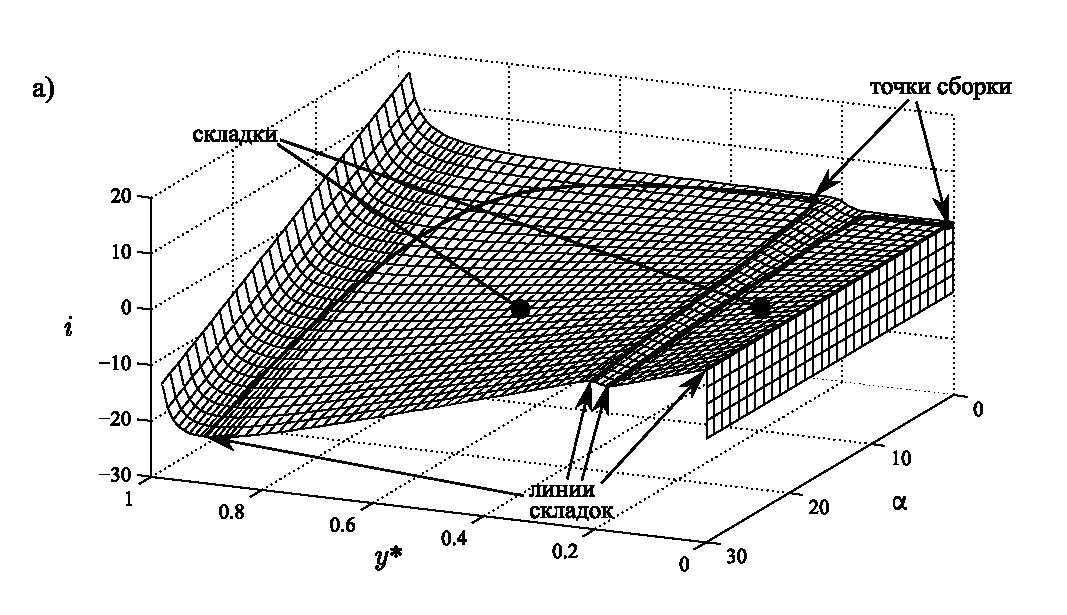
\includegraphics[width=1.0\textwidth]{analysis_origin_solution_surface}}
    \makebox[\textwidth][c]{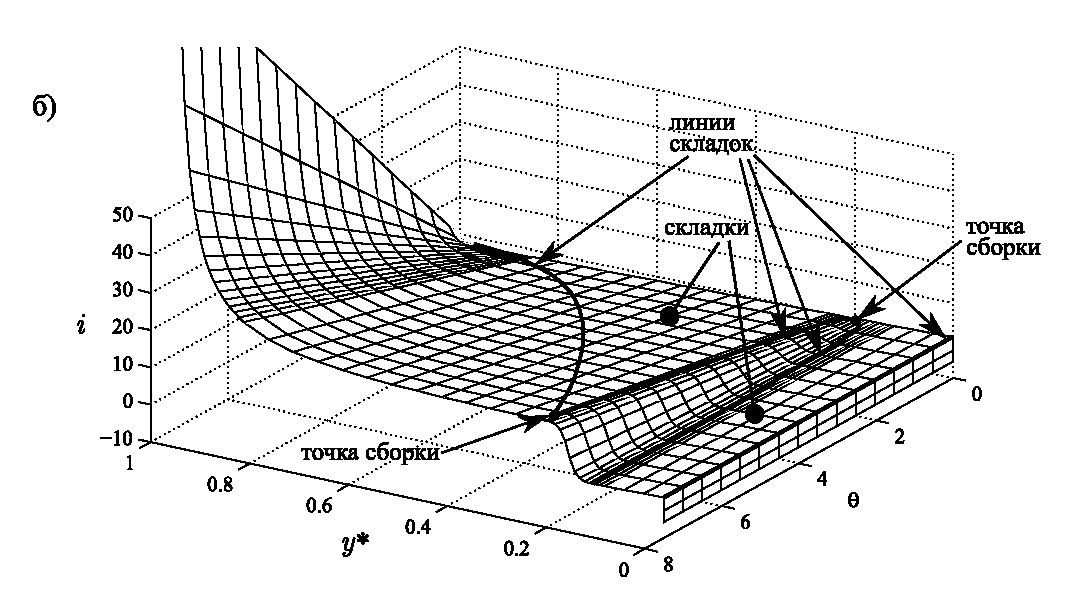
\includegraphics[width=1.0\textwidth]{analysis_origin_solution_surface_p2}}
    \caption{Поверхность решений системы~\eqref{eq:simple_microensemble_model}, построенная вариацией параметров: а) $\alpha$ и $\scalar{i}$ при $\theta = 1, \mu = 0,75$; б) $\theta$ и $\scalar{i}$ при $\alpha = 3,5, \mu = 0,75$.}
    \label{fig:analysis_origin_solution_surface}
\end{figure}

Как было показано в~\autoref{subsection:analysis_sigm}, $s$-образная складка порождает в пространстве параметров модели область би-стабильности, поэтому на объединении множеств~\eqref{eq:origin_stability_area} гарантированно существует два устойчивых решения системы~\eqref{eq:simple_microensemble_model}. Однако, как было отмечено в начале данного подраздела (\seefigure~\ref{fig:analysis_origin_equilibriums}г), при наложении складок возникает область существования трёх устойчивых решений --- это соответствует ситуации, когда первые два множества из объединения~\eqref{eq:origin_stability_area} пересекаются, \ie когда $\alpha_{2} < \alpha < \alpha_{3}$ и $\scalar{i}_{high}^{-} < \scalar{i}_{low}^{+}$. Для определения точных границ данной области решим последнее неравенство, раскрыв переменную $\scalar{i}_{high}^{-}$ согласно~\eqref{eq:origin_stability_bounds_i} и отметив, что $\scalar{i}_{low}^{+} = \mu \theta \cdot u_{01}$:
\begin{equation}
    \nonumber
    -\alpha \left(1 - \sqrt{z_{12}\mu\theta/\alpha}\right) + \mu \theta \left(k_{12} + z_{12} \big/ \sqrt{z_{12}\mu\theta/\alpha} \right) < \mu \theta u_{01}.
\end{equation}
Домножая неравенство на величину $z_{12} / \alpha$ и обозначая как $x = \sqrt{z_{12}\mu\theta/\alpha}$, перепишем его в следующем виде:
\begin{equation}
    \nonumber
    \begin{aligned}
        -z_{12} (1 - x) + x^{2} (k_{12} + z_{12} / x)   &< u_{01} x^{2}, \\
        (k_{12} - u_{01}) x^{2} + 2 z_{12} x - z_{12}   &< 0. \\
    \end{aligned}
\end{equation}
Решением получившегося равенства будут корни:
\begin{equation}
    \nonumber
    x_{1,2} = -\left(z_{12} / (k_{12} - u_{01})\right) \pm \sqrt{\left(z_{12} / (k_{12} - u_{01})\right)^{2} + \left(z_{12} / (k_{12} - u_{01})\right)}.
\end{equation}
которые приближённо будут равны: $x_{1} \approx 0,2779$ и $x_{2} \approx -0,6257$. Учитывая, что по определению $x > 0$, корень $x_{2}$ лежит в области недопустимых значений. Таким образом, переобозначив оставшийся корень как $s_{12} = x_{1}$ и используя определение переменной $x$, мы получим решение в виде:
\begin{equation}
    %\label{eq:origin_bifurcation_tristability}
    \nonumber
    \mu \theta / \alpha < s_{12}^{2} / z_{12}.
\end{equation}

В этом случае точка бифуркации, при которой возникает область существования трёх устойчивых решений, будет равна:
\begin{equation}
    \label{eq:origin_bifurcation_alpha_ext}
    \alpha_{4} = \mu \theta \cdot z_{12} / s_{12}^{2} \approx \mu \theta \cdot 4,75,
\end{equation}
а сама область три-стабильности, учитывая границы множест~\eqref{eq:origin_stability_area}, будет определяться как множество (\seefigure~\ref{fig:analysis_origin_bifurcations}б):
\begin{equation}
    \label{eq:origin_stability_area_ext}
    \{ (\alpha, \scalar{i}) \mid \alpha_{4} < \alpha < \alpha_{3}, \min(i^{-}_{low}, i^{-}_{high}) < \scalar{i} < \max(i^{+}_{low}, i^{+}_{high}) \}.
\end{equation}

Как отмечалось выше, в выражениях~\eqref{eq:origin_stability_bounds_y}, которые определяют точки экстремума кривой решений $F(y)$, параметр $\theta$ входит обратно пропорционально параметру $\alpha$, поэтому бифуркационный анализ относительно параметра $\theta$ даст аналогичные описанным результаты.

Серия бифуркаций типа суперкритическая \inquotes{вилка} продемонстрирована \onfigure~\ref{fig:analysis_origin_bifurcations}в: при монотонном возрастании значения параметра $\theta$ сначала возникает новая точка устойчивого равновесия в дополнение к двум уже существующим, а затем дважды происходит аннигиляция двух из них, в результате чего в системе остаётся всего одна точка устойчивого равновесия (\onfigure~\ref{fig:analysis_origin_bifurcations}г пунктиром обозначены соответствующие при этом значения параметра $i$, обеспечивающие форму изображённой \inquotes{вилки}). Точки бифуркации находятся из тех же соображений, что и бифуркационные точки~\eqref{eq:origin_bifurcation_alpha}, и соответственно равны:
\begin{equation}
    \label{eq:origin_bifurcation_theta}
    \begin{aligned}
        % переобозвать  альфы как high/low^+/-
        \theta_{1} &= \dfrac{(x_{01} + 1)^2}{312 x_{01}} \cdot \alpha / \mu     \approx 3,9 \cdot 10^{7} \cdot \alpha / \mu, \\
        \theta_{2} &= \dfrac{(1 - y_{12})^2}{z_{12}} \cdot \alpha / \mu         \approx 1,56 \cdot \alpha / \mu, \\
        \theta_{3} &= \dfrac{1}{78} \cdot \alpha / \mu                          \approx 1,9 \cdot 10^{-2} \cdot \alpha / \mu.
    \end{aligned}
\end{equation}

Бифуркация типа \inquotes{сборка} изображена \onfigure~\ref{fig:analysis_origin_bifurcations}г: при значениях параметра $\theta$, которые допускают мульти-стабильность модели, количество устойчивых решений в системе~\eqref{eq:simple_microensemble_model} будет зависеть от значения параметра $\scalar{i}$. В данном случае область гарантированного существования двух устойчивых решений, которая определяется аналогично множествам~\eqref{eq:origin_stability_area}, будет равна:
\begin{equation}
    \nonumber
    \begin{aligned}
        &\{ (\theta, \scalar{i}) \mid \theta_{3} < \theta < \theta_{1}, i^{-}_{low} < \scalar{i} < i^{+}_{low} \}, \\
        &\{ (\theta, \scalar{i}) \mid \theta_{3} < \theta < \theta_{2}, i^{-}_{high} < \scalar{i} < i^{+}_{high} \}, \\
        &\{ (\theta, \scalar{i}) \mid \theta \le \theta_{3}, i^{+}_{low} < \scalar{i} < i^{-}_{high} \}. \\
    \end{aligned}
\end{equation}

Соответствующая поверхность решений системы~\eqref{eq:simple_microensemble_model} продемонстрированна \onfigure~\ref{fig:analysis_origin_solution_surface}б, где отмечены области $s$-образных складок, а срезы этой поверхности, привязанные к плоскости параметров, изображены \onfigure~\ref{fig:model_origin_configurations_by_theta}. При этом точки сборки, как следует из бифуркационных значений параметра $\theta$, будут определятся как:
\begin{equation}
    \nonumber
    \begin{aligned}
    &(\theta, \scalar{i}) = \left( \dfrac{(x_{01} + 1)^2}{312 x_{01}} \cdot \alpha / \mu ,\ \dfrac{(x_{01} + 1)^2 \,u_{01}}{312 x_{01}} \cdot \alpha \right), \\
    &(\theta, \scalar{i}) = \left( \dfrac{(1 - y_{12})^2}{z_{12}} \cdot \alpha / \mu     ,\ \minus y_{12} \cdot \alpha + \dfrac{(1 - y_{12})^2 \,u_{01}}{z_{12}} \cdot \alpha \right) , \\
    &(\theta, \scalar{i}) = \left( \dfrac{1}{78} \cdot \alpha / \mu                      ,\ \minus 0,1768 \cdot \alpha \right).
    \end{aligned}
\end{equation}

Область же существования трёх устойчивых решений, определяемая аналогично множеству~\eqref{eq:origin_stability_area_ext}, будет задана следующим выражением (\seefigure~\ref{fig:analysis_origin_bifurcations}г):
\begin{equation}
    \nonumber
    \{ (\theta, \scalar{i}) \mid \theta_{3} < \theta < \theta_{4}, \min(i^{-}_{low}, i^{-}_{high}) < \scalar{i} < \max(i^{+}_{low}, i^{+}_{high}) \},
\end{equation}
где величина $\theta_{4}$, определяемая аналогично величине~\eqref{eq:origin_bifurcation_alpha_ext}, соответствует точке в пространстве параметров, где возникает эффект наложения $low$- и $high$-складок, и равна:
\begin{equation}
    \label{eq:origin_bifurcation_theta_ext}
    \theta_{4} = \dfrac{s_{12}^{2}}{z_{12}} \cdot \alpha / \mu \approx 2,1 \cdot 10^{-1} \cdot \alpha / \mu.
\end{equation}

Если объединить результаты, полученные для параметров $\alpha$ и $\theta$, то область существования двух устойчивых решений системы~\eqref{eq:simple_microensemble_model}, как следует из выражений~\eqref{eq:origin_bifurcation_alpha} и~\eqref{eq:origin_bifurcation_theta}, будет определяться в пространстве этих параметров условием $\alpha \big/ \theta > 312 \mu x_{01} \big/ (x_{01} + 1)^{2}$, а область существования трёх устойчивых состояний, как следует из выражений~\eqref{eq:origin_bifurcation_alpha_ext} и~\eqref{eq:origin_bifurcation_theta_ext}, -- условием $z_{12} \mu \big/ s_{12}^{2} < \alpha \big/ \theta < 78 \mu$. Данное пространство изображено \onfigure~\ref{fig:analysis_origin_alpha_vs_theta}: соответствующая крайне узкому диапазону значений область моно-стабильности не закрашена; соответствующая $low$- и $high$- складкам область би-стабильности отмечана диагональной штриховкой справа-налево, а область би-стабильности $broad$-складки --- диагональной штриховкой слева-направо; область три-стабильности отмечена двойной штриховкой. Причём пунктирная линия, определяемая условием $\alpha \big/ \theta = z_{12} \mu \big/ (1 - y_{12})^2$, задаёт в правой полуплоскости область существования $high$-складки и соответствующих ей точек устойчивого равновесия.

\IncludeFigure[ht]{analysis_origin_alpha_vs_theta}{Области моно-, би- и три-стабильности системы~\eqref{eq:simple_microensemble_model} на плоскости параметров $\alpha$ и $\theta$ (закрашены без, одинарной и двойной штриховкой соотвественно): а) в линейном масштабе; б) в логарифмическом масштабе.}

Как и в случае с \acr{SAF}-моделью, данные области мульти-стабильности определяют необходимое, но не достаточное условие существования нескольких устойчивых точек в модели --- как отмечалось при выводе величин $i_{low}^{\pm}$ и $i_{high}^{\pm}$~\eqref{eq:origin_stability_bounds_i}, в каждой из областей значение параметра $\scalar{i}$ должно лежать в определённом интервале значений. Таким образом, область существования не менее двух точек устойчивого равновесия будет определяться объединением множеств:
\begin{equation}
    \nonumber
    \begin{aligned}
    &\{(\alpha, \theta, \scalar{i}) \mid 312 \mu x_{01} \big/ (x_{01} + 1)^{2} < \alpha \big/ \theta < 78 \mu, i^{-}_{low} < \scalar{i} < i^{+}_{low} \}, \\
    &\{(\alpha, \theta, \scalar{i}) \mid z_{12} \mu \big/ (1 - y_{12})^2 < \alpha \big/ \theta < 78 \mu, i^{-}_{high} < \scalar{i} < i^{+}_{high} \}, \\
    &\{(\alpha, \theta, \scalar{i}) \mid \alpha \big/ \theta \ge 78 \mu, i^{+}_{low} < \scalar{i} < i^{-}_{high} \}. \\
    \end{aligned}
\end{equation}
При этом подмножество данной области, которому соответствует область существования трёх точек устойчивого равновесия, будет определяться следующим образом:
\begin{equation}
    \nonumber
    \{(\alpha, \theta, \scalar{i}) \mid z_{12} \mu \big/ s_{12}^{2} < \alpha \big/ \theta < 78 \mu, \min(i^{-}_{low}, i^{-}_{high}) < \scalar{i} < \max(i^{+}_{low}, i^{+}_{high}) \}.
\end{equation}

%==============================================================================
\subsection{Обобщение на семейство функций активации}  \label{subsection:analysis_custom}

Общим для рассмотренных выше \acr{SAF}- и \acr{OAF}-моделей является зависящее от значений параметров $\alpha$ и $\theta$ наличие или же отсутствие на графике решений системы~\eqref{eq:simple_microensemble_model} $s$-образных складок, которые обуславливают наличие областей мульти-стабильности в модели. Естественно предположить, что и \textit{сигмоидальная}, и \textit{оригинальная} функция активации являются лишь частными случаями из целого семейства функций активации, использование которых в модели микроансамбля будет приводить к появлению характерных свойств.

Однако, прежде чем переходить к непосредственному обобщению результатов на семейство активационных функций, рассмотрим и докажем вспомогательную лемму, предполагая, что все наши рассуждения относятся к рассмотрению вещественных функций вещественного аргумента.
\begin{Lemma}
    Пусть функция $f(x)$, заданная на всей числовой оси, является неубывающей, ограниченной и дифференцируемой почти всюду функцией, причём $\exists\, x_{1}, x_{2} \in \specialset{R} \,:\, f(x_{1}) \ne f(x_{2})$, тогда для $\forall\,a,b \in \specialset{R}^{+}$ и $\forall\,c \in \specialset{R}$ существует такое $V \in \specialset{R}$, что функция $F(x) = a f(x) - b x + c$:
    \begin{itemize}
        \item[-] при $b/a \le V$ не будет иметь точек локального экстремума;
        \item[-] при $b/a > V$ будет иметь точки локального экстремума, а их количество будет кратно двум.
    \end{itemize}
\end{Lemma}
\begin{Proof}
    \ldots
\end{Proof}

\begin{Theorem}
    Пусть функция активации $f(x)$ является неубывающей, ограниченной и дифференцируемой почти всюду функцией, причём $\exists\, x_{1}, x_{2} \in \specialset{R} \,:\, f(x_{1}) \ne f(x_{2})$, тогда существует такое $V \in \specialset{R}$, что заданная дифференциальным уравнением~\eqref{eq:simple_microensemble_model_plain} модель нейрона:
    \begin{itemize}
        \item[-] при $\mu \theta / \alpha \le V$ будет имеет ровно одну точку устойчивого равновесия;
        \item[-] при $\mu \theta / \alpha > V$ может иметь одну или более точек устойчивого равновесия, а их точное число зависит от значения параметра $\scalar{i}$.
    \end{itemize}
\end{Theorem}
\begin{Proof}
    \ldots
\end{Proof}

%Легко видеть, что \textit{сигмоидальная} и \textit{оригинальная} функции удовлетворяют условиям \ldots

%==============================================================================
%                       Характерные свойства и динамика
%==============================================================================
%\newpage
\section{Характерные свойства и динамика} \label{section:neuron_dynamic}

%Стоит отметить, что несмотря на отсутствие точного аналитического решения системы~\eqref{eq:simple_microensemble_model}, найденные в предыдущем разделе бифуркационные точки, с одной стороны, позволяют подобрать начальные неизменяемые параметры модели $\mu$ и $\alpha$, а с другой, оценить качественные изменения модели при вариации значений параметра $\theta$.

%==============================================================================
\subsection{Определения и свойства}

\begin{Definition}
    \textit{Мягким режимом (конфигурацией)} функционирования микроансамбля будем называть такое его состояние, при котором описывающая его динамическая система является моно-стабильной...
\end{Definition}

\begin{Definition}
    \textit{Жёстким режимом (конфигурацией)} функционирования микроансамбля будем называть такое его состояние, при котором описывающая его динамическая система является мульти-стабильной...
\end{Definition}

\begin{Definition}
    Определим \textit{степень жёсткости} $R[A]$ микроансамбля $A$ как ..., т.е. как величину: $$ R[A] = \max\limits_{\alpha,\theta,\mu,\scalar{i}} \left| \left\{ \scalar{y_{i}} \mid F(\scalar{y_{i}}) = 0 \right\} \right| - 1. $$
\end{Definition}

Заметим, что в этом случае \textit{мягкому режиму} соответствует конфигурация микроансамбля с нулевой степенью жёсткости. Таким образом, можно ввести отношение порядка между конфигурациями микроансамбля.

\begin{Definition}
    Будем говорить, что
\end{Definition}

%\begin{Definition}
%    \textit{Мягким режимом} функционирования микроансамбля будем называть...
%\end{Definition}
%
%\begin{Definition}
%    \textit{Жёстким режимом} функционирования микроансамбля будем называть...
%\end{Definition}

% - определения мягкого и жёсткого режимов + порядок жёсткости n (существование n-стаб. обл.) + отношение более-менее для однопорядковых жёстких систем
% - условия существования мягкого и жёсткого режимов
% - свойства мягкого и жёсткого режимов

%\begin{Statement}
%    \todo{про мягкий режим и условия его существования.}
%\end{Statement}
%
%\begin{Statement}
%    \todo{про жёсткий режим и условия его существования.}
%\end{Statement}
%


%==============================================================================
\subsection{Численное моделирование}

Для выполнения численных экспериментов с рабочей моделью необходимо в первую очередь привести её к эквивалентной дискретной форме, применив один из разностных методов. Для этого в ходе исследований было рассмотрено применение таких классических методов как явный метод Эйлера, модифицированный метод Эйлера с пересчётом (разновидность метода Рунге-Кутты второго порядка точности), а так же явный метод Рунге-Кутты четвёртого порядка точности~\cite{Hairer1990}. Отметим, что при выборе разумного с точки зрения точности и вычислительной эффективности шага дискретизации $h$ использование того или иного метода не вносило существенных изменений в результаты численных экспериментов --- более подробно сравнение методов освещено \inappendix~\ref{appendix:differential_schemes_compare} \inquotes{\nameref{appendix:differential_schemes_compare}}. Поэтому в данной главе для численного моделирования был использован явный метод Эйлера с шагом $h = 0,01$ как наиболее простой в реализации метод.

Таким образом, система~\eqref{eq:simple_microensemble_model}, записанная в дифференциальной форме, приобрела следующий конечно-разностный вид:
\begin{equation}
    \label{eq:simple_microensemble_discrete}
    \begin{cases}
        \scalar{u^{t+1}} = \scalar{u^{t}} + h \cdot ( \alpha\scalar{y^{t}} + \scalar{i^{t}} - \mu\scalar{u^{t}} ), \\ 
        \scalar{y^{t+1}} = f(h(\scalar{u^{t+1}})),
    \end{cases}
\end{equation}
где верхний индекс $t \ge 0$ соответствует некоторому дискретному значению времени и задаёт состояние переменных модели в этот момент времени.


%==============================================================================
%                               Выводы по главе
%==============================================================================
\section{Выводы по главе \thechapter} \label{section:neuron_concls}



